\chapter{Implementacija i korisničko sučelje}
		
		
		\section{Korištene tehnologije i alati}
			
			 \textit U razvoju ove web aplikacije koristili smo mnoge programe za izradu frontend i backend dijela. Backend se odvijao u razvojnoj okolini \textbf{Eclipse}, a logika backend dijela je u programskom jeziku \textbf{Java} i \textbf{Spring Bootu}.
			 \newline Za izradu dijagrama koje smo trebali izraditi u sklopu projekta koristili smo alat \textbf {Astah}. Za implementaciju baze te njeno vođenje koristili smo \textbf{PostgreSQL}.
			 \newline Frontend je napravljen isto tako u Eclipseu, a korištena je \textbf{Bootstrap} biblioteka. 
			 \newline Kao Web poslužitelj koristili smo \textbf{Apache Tomcat} koji je implementiran u Spring Boot.
			 Ažuriranje verzije projekta te dodavanje novih implementacija odvijalo se preko \textbf {Gitlaba}.
			 \newline
			 \newline
			 \noindent
			 \underline{Eclipse}
			 \newline
			 Razvojno okruženje koje se koristi za razne programske jezike.
			 \newline
			 \url{https://www.eclipse.org/downloads/}
			 \newline
			 \newline
			 \underline{Java}
			 \newline
			 Programski jezik opće namjene koji se temelji na klasama te je objektno orijentiran.
			 \newline
			 \url{https://www.oracle.com/technetwork/java/javase/downloads/jdk8-downloads-2133151.html}
			 \newline
			 \newline
			 \underline{Spring Boot}
			 \newline
			 \emph{Open-source framework} koji je temeljen na Javi. Omogućava lakšu izradu Spring aplikacija jer se programer ne mora brinuti o raznim implementacijskim akcijama.
			 \newline
			 \url{https://spring.io/tools3/eclipse}
			 \newline
			 \newline
			 \newpage
			 \noindent
			 \underline{Astah}
			 \newline
			 Alat za modeliranje UML dijagrama koji se može koristiti za sve UML dijagrame obrađene na predmetu.
			 \newline
			 \url{http://astah.net/download}
			 \newline
			 \newline
			 \underline{PostgreSQL}
			 \newline
			 Besplatni izvorni sustav za upravljanje relacijskim bazama. Susreli smo se s njim na predmetu Baze podataka.Dizajniran je za obradu različitih podataka, od pojedinačnih strojeva do skladišta podataka ili web usluga s mnogim istodobnim korisnicima.
			 \newline
			 \url{https://www.postgresql.org/download/}
			 \newline
			 \newline
			 \underline{Apache Tomcat}
			 \newline
			 Tehnologija koja pruža okruženje HTTP web poslužitelja u kojem se Java kod može pokretati.
			 \newline
			 \url{https://tomcat.apache.org/download-80.cgi}
			 \newline
			 \newline
			 
			\eject 
		
	
		\section{Ispitivanje programskog rješenja}
			
			 
	
			
			\subsection{Ispitivanje komponenti}
			\textit{Ispitivanje je provedeno nad korisničkim unosima prilikom registacije i prilikom dodavanja novih objekata u muzej.   }
			
			
			\textit{Prilikom registracije korisnik unosi svoju E-mail adresu. Ta adresa mora biti valjana i ispravnog formata. To znači da mora sadržavati znak @ i da smije sadržavati samo slova i brojeve. Strogo su zabranjeni matematički operatori i ostali simboli koji nisu u abecedi }
			
			\begin{figure}[H]
				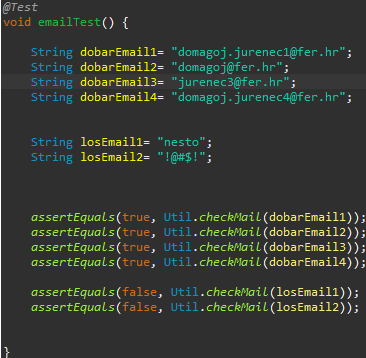
\includegraphics[scale=1]{slike/Junit1.png}
				\centering
				\caption{Ispitivanje različitih formata E-mail adrese}
				\label{fig:promjene}
			\end{figure}
		\newpage
		\textit{Prilikom registracije korisnik unosi svoje korisničko ime. Korisničko ime smije sadržavati brojeve i slova, a ne smije sadržavati razmake i matematičke operatore i ostale simbole koji nisu u abecedi }
		
			\begin{figure}[H]
				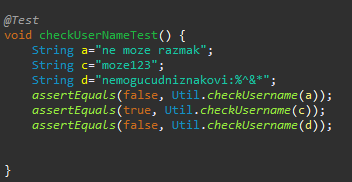
\includegraphics[scale=1]{slike/Junit2.png}
				\centering
				\caption{Ispitivanje različitih formata korisničkog imena}
				\label{fig:promjene}
			\end{figure}
			
			\textit{Prilikom registracije korisnik unosi svoju lozinku. Lozinka mora sadržavati i velika i mala slova i mora imati duljinu od barem 7 znakova }
			
			\begin{figure}[H]
				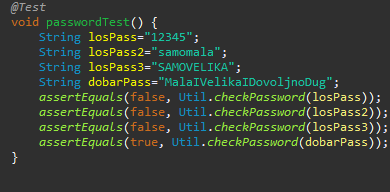
\includegraphics[scale=1]{slike/Junit3.png}
				\centering
				\caption{Ispitivanje različitih formata lozinke}
				\label{fig:promjene}
			\end{figure}
			\newpage
			\textit{Prilikom unosa novog muzejskog objekta unosi se i njegov opis. Opis smije sadržavati slova, brojke, pravopisne znakove i zagrade, a ne smije sadržavati ostale matematičke operatore i simbole koji nisu u abecedi }
			
			\begin{figure}[H]
				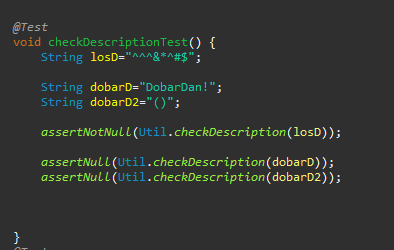
\includegraphics[scale=1]{slike/Junit4.png}
				\centering
				\caption{Ispitivanje formata opisa muzejskih objekata}
				\label{fig:promjene}
			\end{figure}
		
			\textit{Prilikom unosa novog muzejskog objekta unosi se njegov naslov. Naslov smije sadržavati slova, brojke i pravopisne znakove, a ne smije sadržavati  matematičke operatore i ostale simbole koji nisu u abecedi }
		
			\begin{figure}[H]
				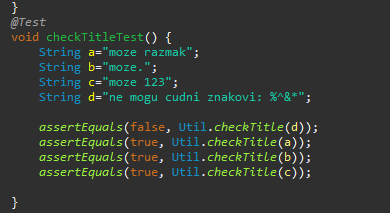
\includegraphics[scale=1]{slike/Junit5.png}
				\centering
				\caption{Ispitivanje formata naslova muzejskih objekata}
				\label{fig:promjene}
			\end{figure}
		
		
			\newpage
			\textit{Prilikom interakcije s aplikacijom možemo napraviti zabranjenu radnju. Aplikacija tada korisniku daje do znanja da je počinjena greška te zanemaruje krivu naredbu. Ukoliko je naredba ispravna, aplikacija ju izvršava te nastavlja s radom. Ispitivanjem utvrđujemo da se aplikacija u svakom trenutku ponaša ispravno.  }
		
			\begin{figure}[H]
				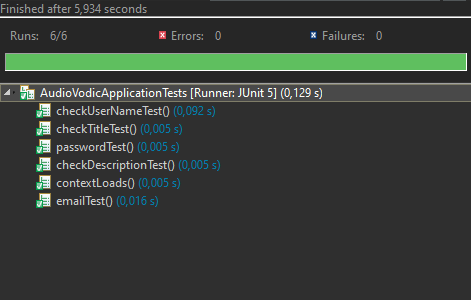
\includegraphics[scale=1]{slike/prolazni_testovi.png}
				\centering
				\caption{Aplikacija ispravno reagira na sve unose}
				\label{fig:promjene}
			\end{figure}
		
			
			
			
			
			\newpage
			\subsection{Ispitivanje sustava}
			
			 \textit{\textbf{Ispitni slučaj 1: Dodavanje novog muzejskog objekta}}
			 \newline
			 \textit{\textbf{Ulaz:}}
			 \begin{packed_enum}	
			 	\item $<$Otvaranje početne stranice u web pregledniku.$>$
			 	\item $<$Odabir opcije za dodavanje muzejskog objekta.$>$
			 	\item $<$Ispunjavanje formulara s podatcima o muzejskom objektu.$>$
			 	\item $<$Pritisak na gumb za dodavanje muzejskog objekta.$>$
			 \end{packed_enum}
			 \textit{\textbf{Očekivani rezultat:}}
			 \begin{packed_enum}
				 \item $<$Prikazuje se web stranica sa svim muzejskim objektima i opcijom dodavanja novog muzejskog objekta.$>$
				 \item $<$Prikazuje se formular za dodavanje muzejskog objekta.$>$
				 \item $<$Ako je formular ispravno popunjen dodaje se novi muzejski objekt i prikazuje početna stranica.$>$ 
			 \end{packed_enum}
			 \textit{\textbf{Rezultat:} Novi muzejski objekt se dodaje i prikazuje se web stranica sa svim muzejskim objektima ili sustav dojavljuje pogrešku.
			 \newline}
			 \begin{figure}[H]
			 	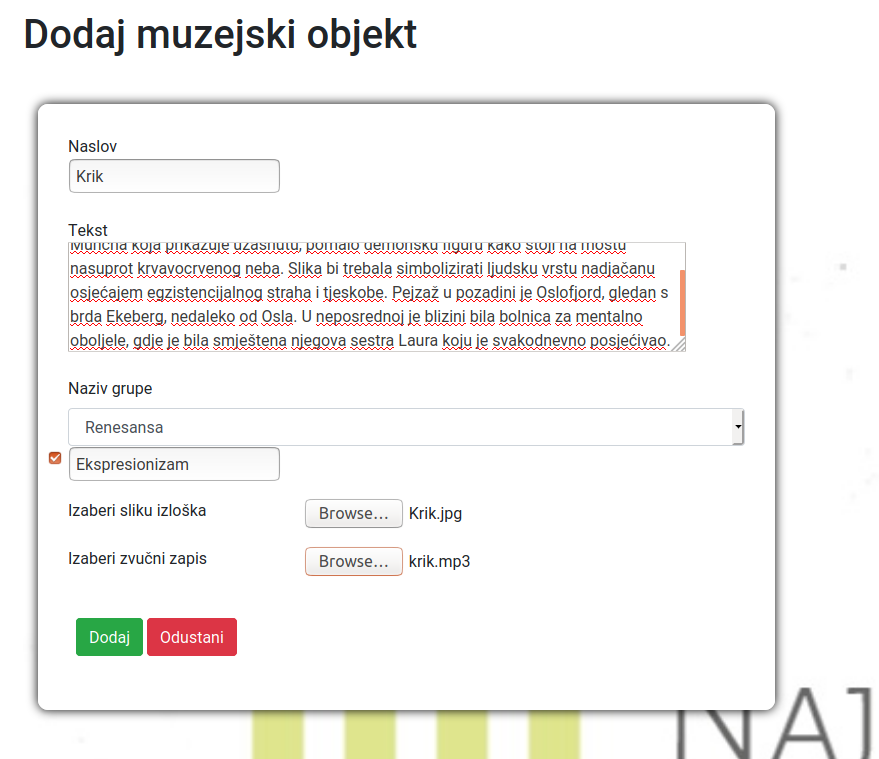
\includegraphics[scale=0.25]{slike/dodavanje1.png}
			 	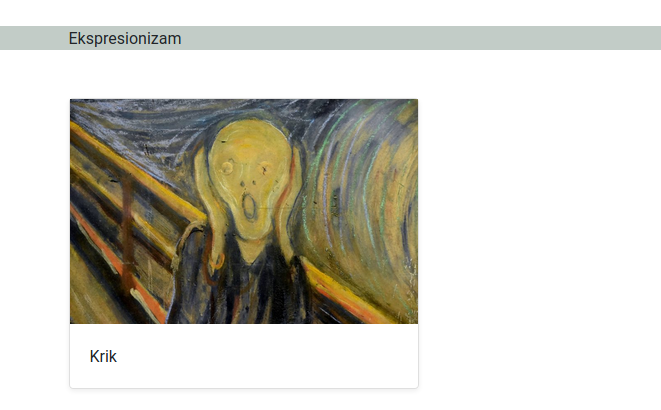
\includegraphics[scale=0.25]{slike/dodavanje2.png}
			 	\centering
			 	\caption{Dodavanje muzejskog objekta}
			 	\label{fig:promjene}
			 \end{figure}
		 
		 
		 
		 	 \textit{\textbf{Ispitni slučaj 2: Detaljniji prikaz muzejskog objekta}}
		 	 \newline
		 	 \textit{\textbf{Ulaz:}}
		 	 \begin{packed_enum}	
		 	 	\item $<$Otvaranje početne stranice u web pregledniku.$>$
		 	 	\item $<$Odabir muzejskog objekta.$>$
		 	 \end{packed_enum}
		 	 \textit{\textbf{Očekivani rezultat:}}
		 	 \begin{packed_enum}
		 	 	\item $<$Prikazuje se web stranica sa svim muzejskim objektima.$>$
		 	 	\item $<$Prikazuje se web stranica s detaljnim prikazom muzejskog objekta.$>$
		 	 \end{packed_enum}
		 	 \textit{\textbf{Rezultat:} Korisniku se uspješno prikazuje muzejski objekt ili sustav dojavljuje pogrešku.
		 	 \newline}
		 	 \begin{figure}[H]
		 	 	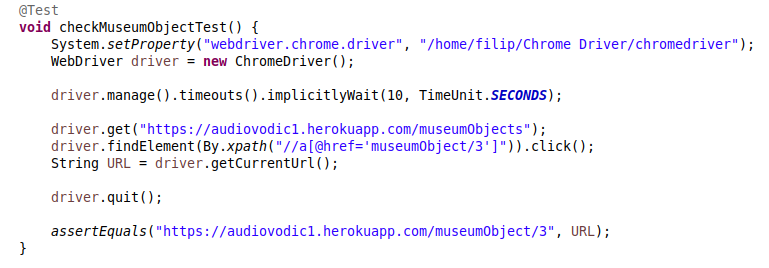
\includegraphics[scale=0.62]{slike/checkMuseumObjectTest.png}
		 	 	\centering
		 	 	\caption{Detaljniji prikaz muzejskog objekta}
		 	 	\label{fig:promjene}
		 	 \end{figure}
	 	 
	 	 
	 	 	 \textit{\textbf{Ispitni slučaj 3: Prijava korisnika}}
	 	 	 \newline
	 	 	 \textit{\textbf{Ulaz:}}
	 	 	 \begin{packed_enum}	
	 	 	 	\item $<$Otvaranje početne stranice u web pregledniku.$>$
	 	 	 	\item $<$Odabir opcije za prijavu.$>$
	 	 	 	\item $<$Ispunjavanje formulara za prijavu.$>$
	 	 	 	\item $<$Pritisak na gumb za prijavu.$>$
	 	 	 \end{packed_enum}
	 	 	 \textit{\textbf{Očekivani rezultat:}}
	 	 	 \begin{packed_enum}
	 	 	 	\item $<$Prikazuje se web stranica sa svim muzejskim objektima.$>$
	 	 	 	\item $<$Prikazuje formular za prijavu.$>$
	 	 	 	\item $<$Ako je formular ispravno popunjen korisnik je uspješno prijavljen te se prikazuje početna stranica.$>$ 
	 	 	 \end{packed_enum}
	 	 	 \textit{\textbf{Rezultat:} Korisnik se uspješno prijavljuje ili mora ponovo ispuniti formular.
	 	 	 	\newline}
	 	 	 \begin{figure}[H]
	 	 	 	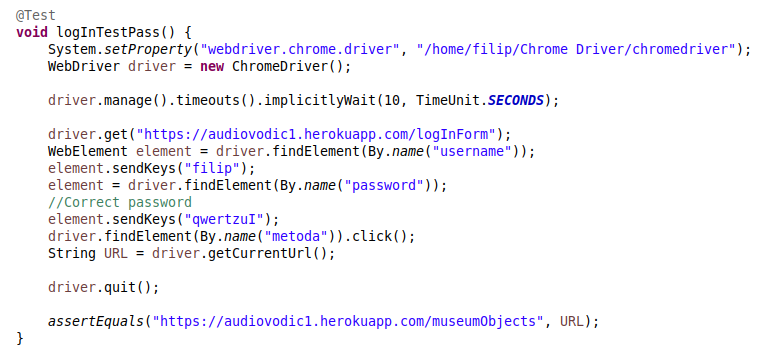
\includegraphics[scale=0.25]{slike/logInTestPass.png}
	 	 	 	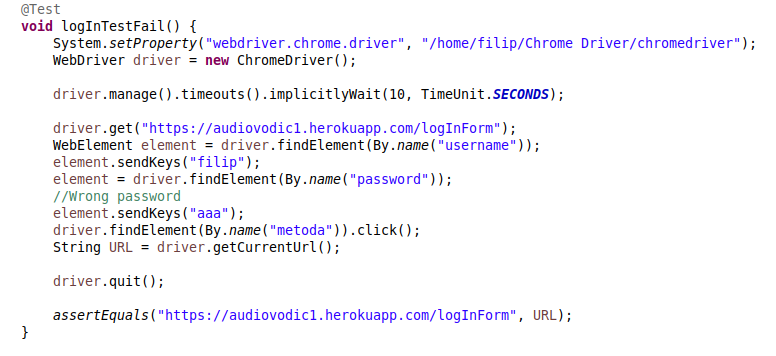
\includegraphics[scale=0.25]{slike/logInTestFail.png}
	 	 	 	\centering
	 	 	 	\caption{Prijava korisnika}
	 	 	 	\label{fig:promjene}
	 	 	 \end{figure}
 	 	 
 	 	 
 	 	 	 \textit{\textbf{Ispitni slučaj 4: Registracija korisnika}}
 	 	 	 \newline
 	 	 	 \textit{\textbf{Ulaz:}}
 	 	 	 \begin{packed_enum}	
 	 	 	 	\item $<$Otvaranje početne stranice u web pregledniku.$>$
 	 	 	 	\item $<$Odabir opcije za prijavu.$>$
 	 	 	 	\item $<$Odabir opcije za izradu novog korisničkog računa.$>$
 	 	 	 	\item $<$Ispunjavanje formulara za registraciju.$>$
 	 	 	 	\item $<$Pritisak na gumb za izradu računa.$>$
 	 	 	 \end{packed_enum}
 	 	 	 \textit{\textbf{Očekivani rezultat:}}
 	 	 	 \begin{packed_enum}
 	 	 	 	\item $<$Prikazuje se web stranica sa svim muzejskim objektima.$>$
 	 	 	 	\item $<$Prikazuje formular za prijavu.$>$
 	 	 	 	\item $<$Prikazuje formular za registraciju.$>$
 	 	 	 	\item $<$Ako je formular ispravno popunjen korisnik je uspješno prijavljen te se prikazuje početna stranica.$>$ 
 	 	 	 	\item $<$Čeka se potvrda korisnika putem email adrese.$>$ 
 	 	 	 \end{packed_enum}
 	 	 	 \textit{\textbf{Rezultat:} Korisnik se uspješno registrira ili mora ponovo ispuniti formular.
 	 	 	 	\newline}
 	 	 	 \begin{figure}[H]
 	 	 	 	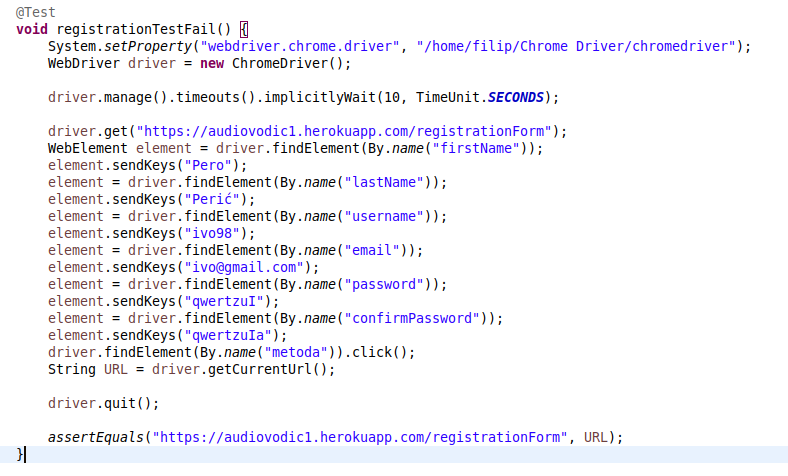
\includegraphics[scale=0.62]{slike/registrationTestFail.png}
 	 	 	 	\centering
 	 	 	 	\caption{Registracija korisnika}
 	 	 	 	\label{fig:promjene}
 	 	 	 \end{figure}
  	 	 
  	 	 	\begin{figure}[H]
  	 	 		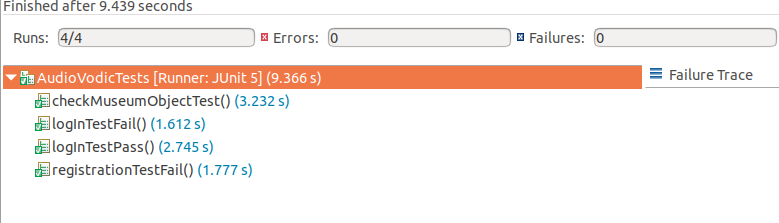
\includegraphics[scale=0.62]{slike/testoviRez.png}
  	 	 		\centering
  	 	 		\caption{Rezultati testova}
  	 	 		\label{fig:promjene}
  	 	 	\end{figure}
			
			\eject 
		
		
		\section{Dijagram razmještaja}
			
			\begin{figure}[H]
				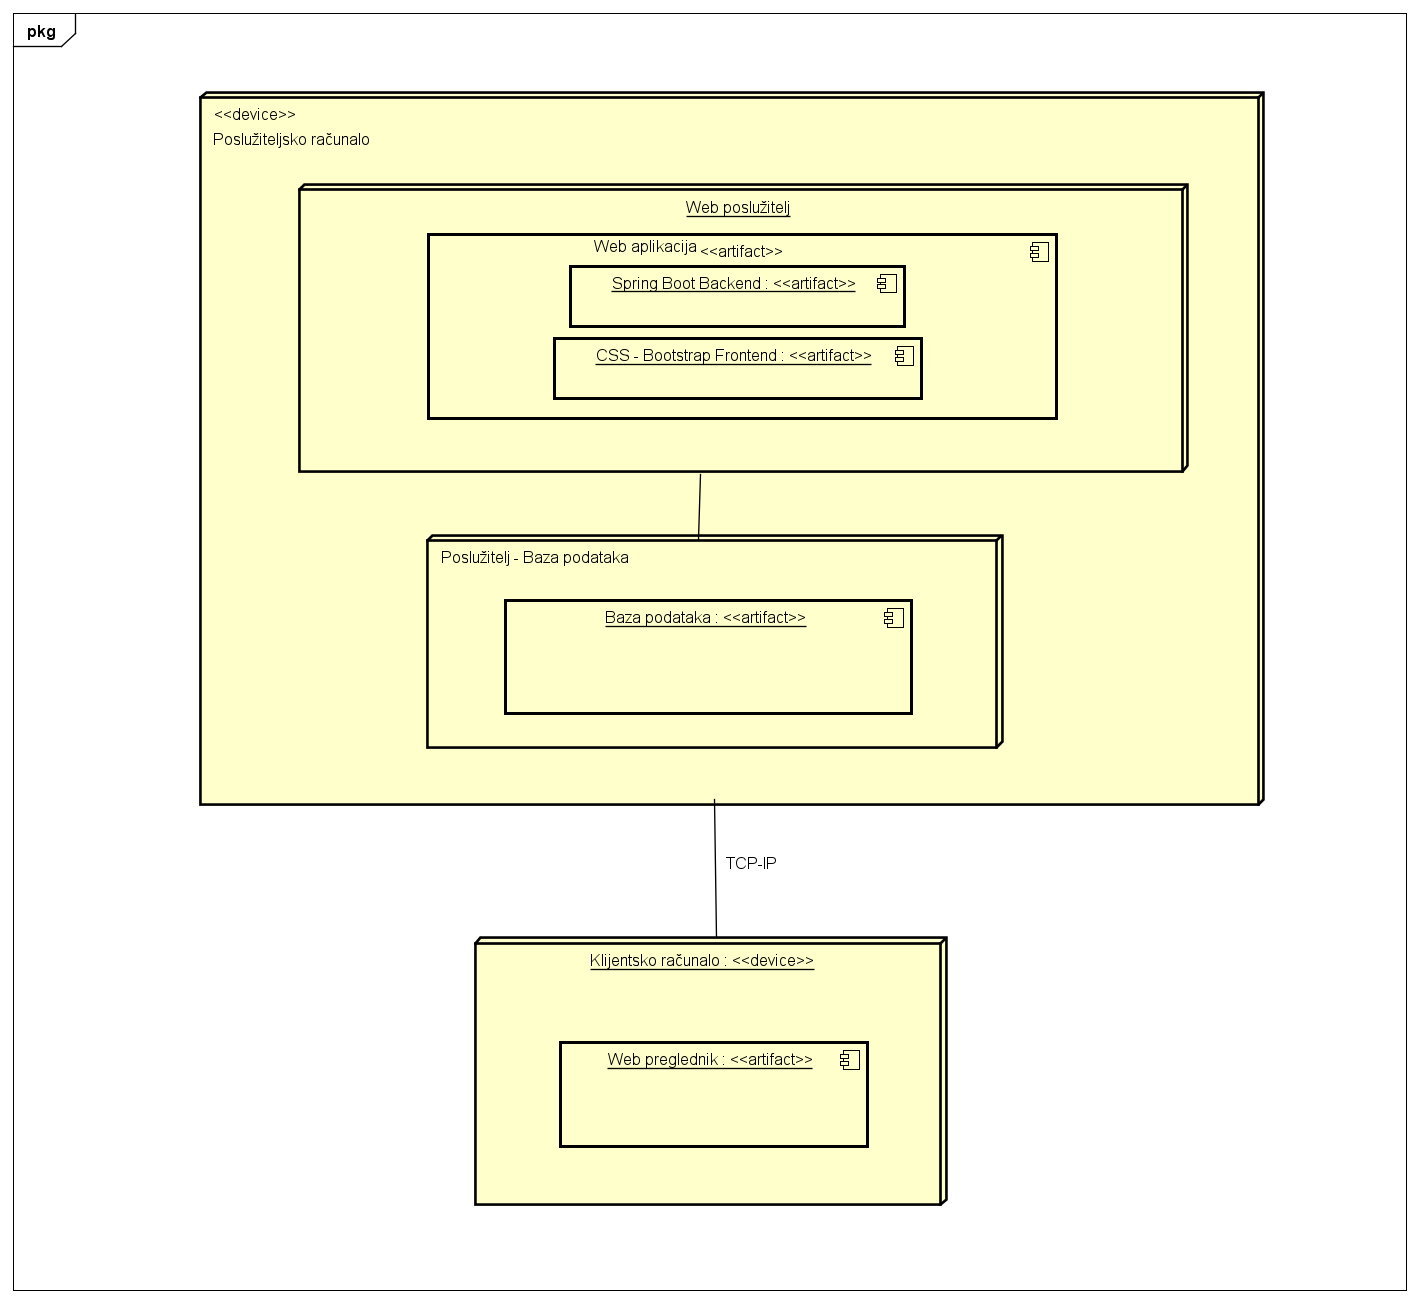
\includegraphics[scale=0.42]{slike/Dijagram_razmjestaja.png}
				\centering
				\caption{Dijagram razmještaja}
				\label{fig:promjene}
			\end{figure}
			
			\textit Dijagram razmještaja je općenito dijagram koji pokazuje hardverske procesore ili čvorove, poveznice komunikacije između njih te softverske datoteke koje se nalaze na tom hardveru. U stvaranju naše web aplikacije, posao smo podijelili na Backend i Frontend, te smo to prikazali artefaktima na poslužiteljskom računalu. Njega smo povezali TCP-IP vezom s klijentskim računalom preko kojeg se pristupa našoj aplikaciji. Važno je istaknuti i bazu podataka na ovom dijagramu u kojem spremamo razne bitne podatke, među kojima su naravno i korisnički podatci. 
			
			\eject
		
		\section{Upute za puštanje u pogon}
		
			 \textit{Kako bi pustili aplikaciju u pogon, potrebno je napraviti deploy. U našem slučaju taj deploy smo napravili na Heroku. 
		  	 \newline
		  	 Kako bi napravili deploy aplikacije na Heroku potrebno je napraviti korisnički račun. Korisnički račun moguće je napraviti na sljedećem linku: \url{https://signup.heroku.com/}. Nakon što se napravi korisnički račun, na mail adresu koja je upisana dobije se link na koji se mora kliknuti kako bi se potvrdio račun i postavila lozinka.}
			 
			 \begin{figure}[H]
			 	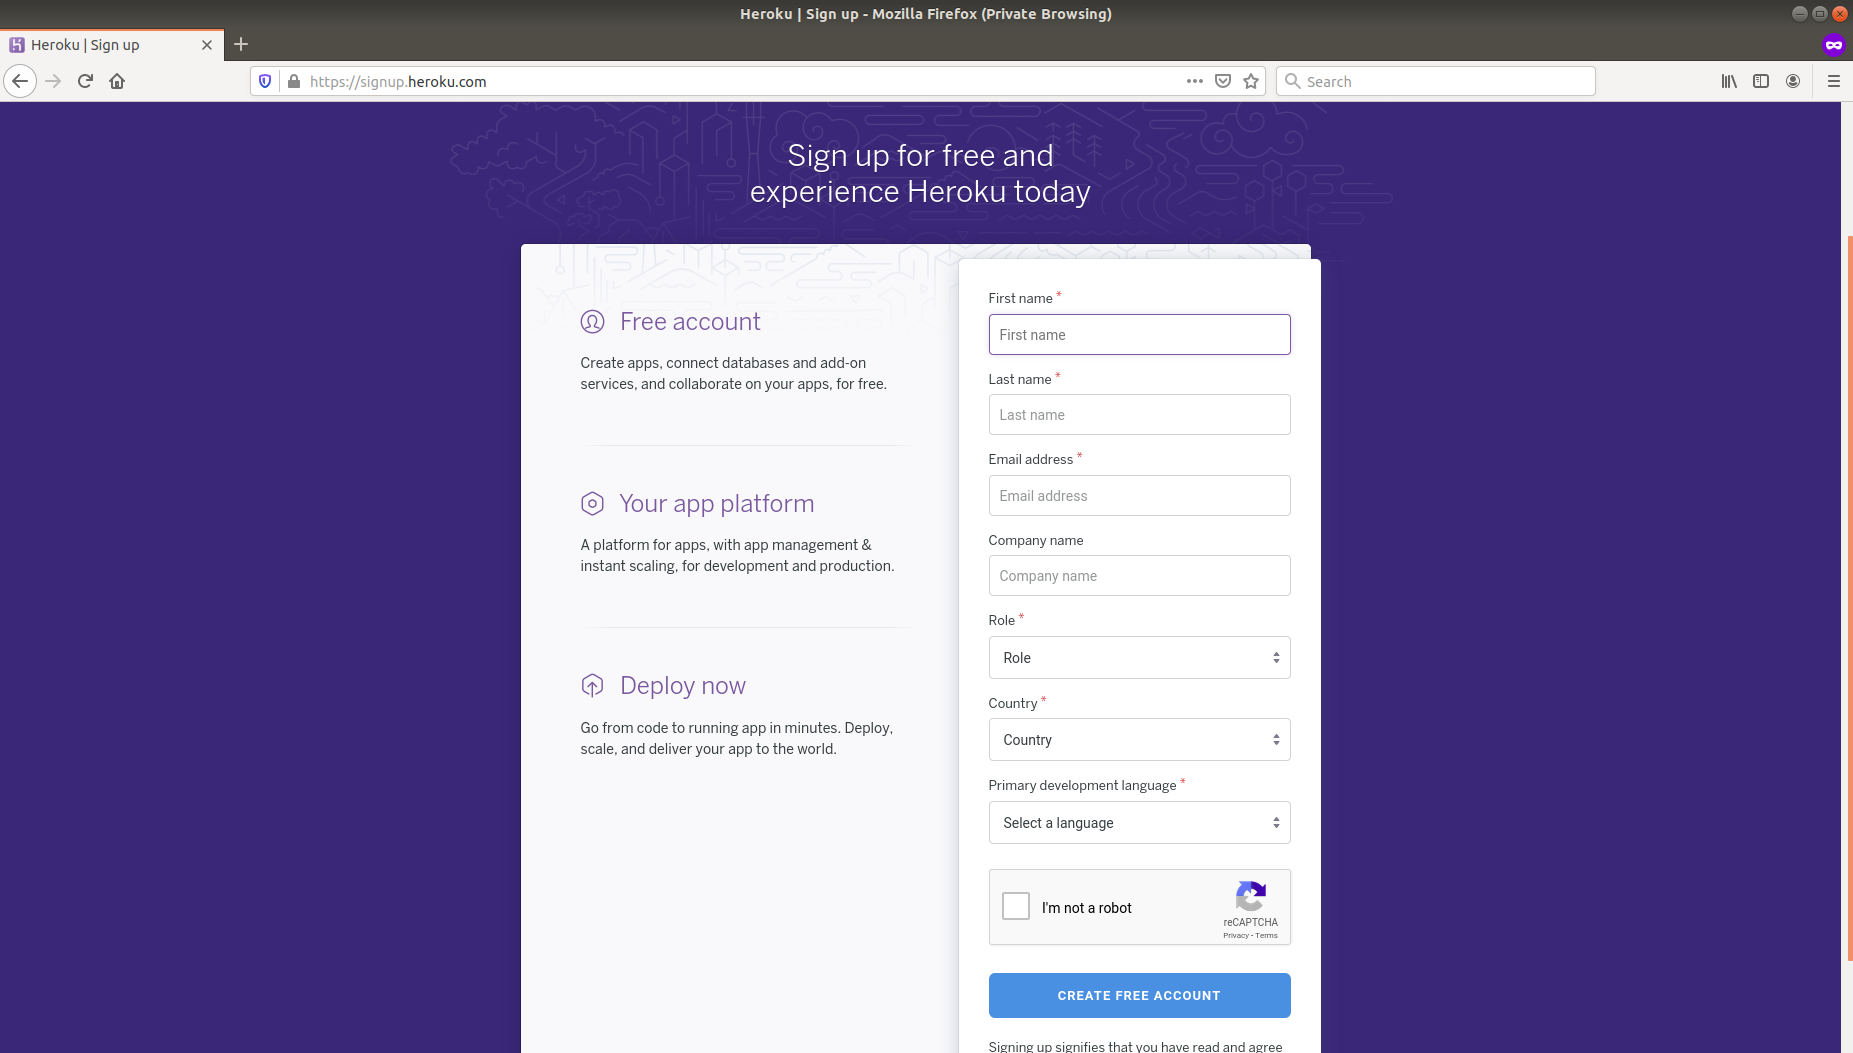
\includegraphics[scale=0.25]{slike/regHeroku.png}
			 	\centering
			 	\caption{Izrada korisničkog računa}
			 	\label{fig:promjene}
			 \end{figure}
		 
		 	\newpage
			 \textit{Slijedeći korak je instalirati heroku CLI. Heroku CLI možete instalirati na različitim operacijskim sustavima (Linux, Windows, macOs).}
			 
			 \begin{figure}[H]
			 	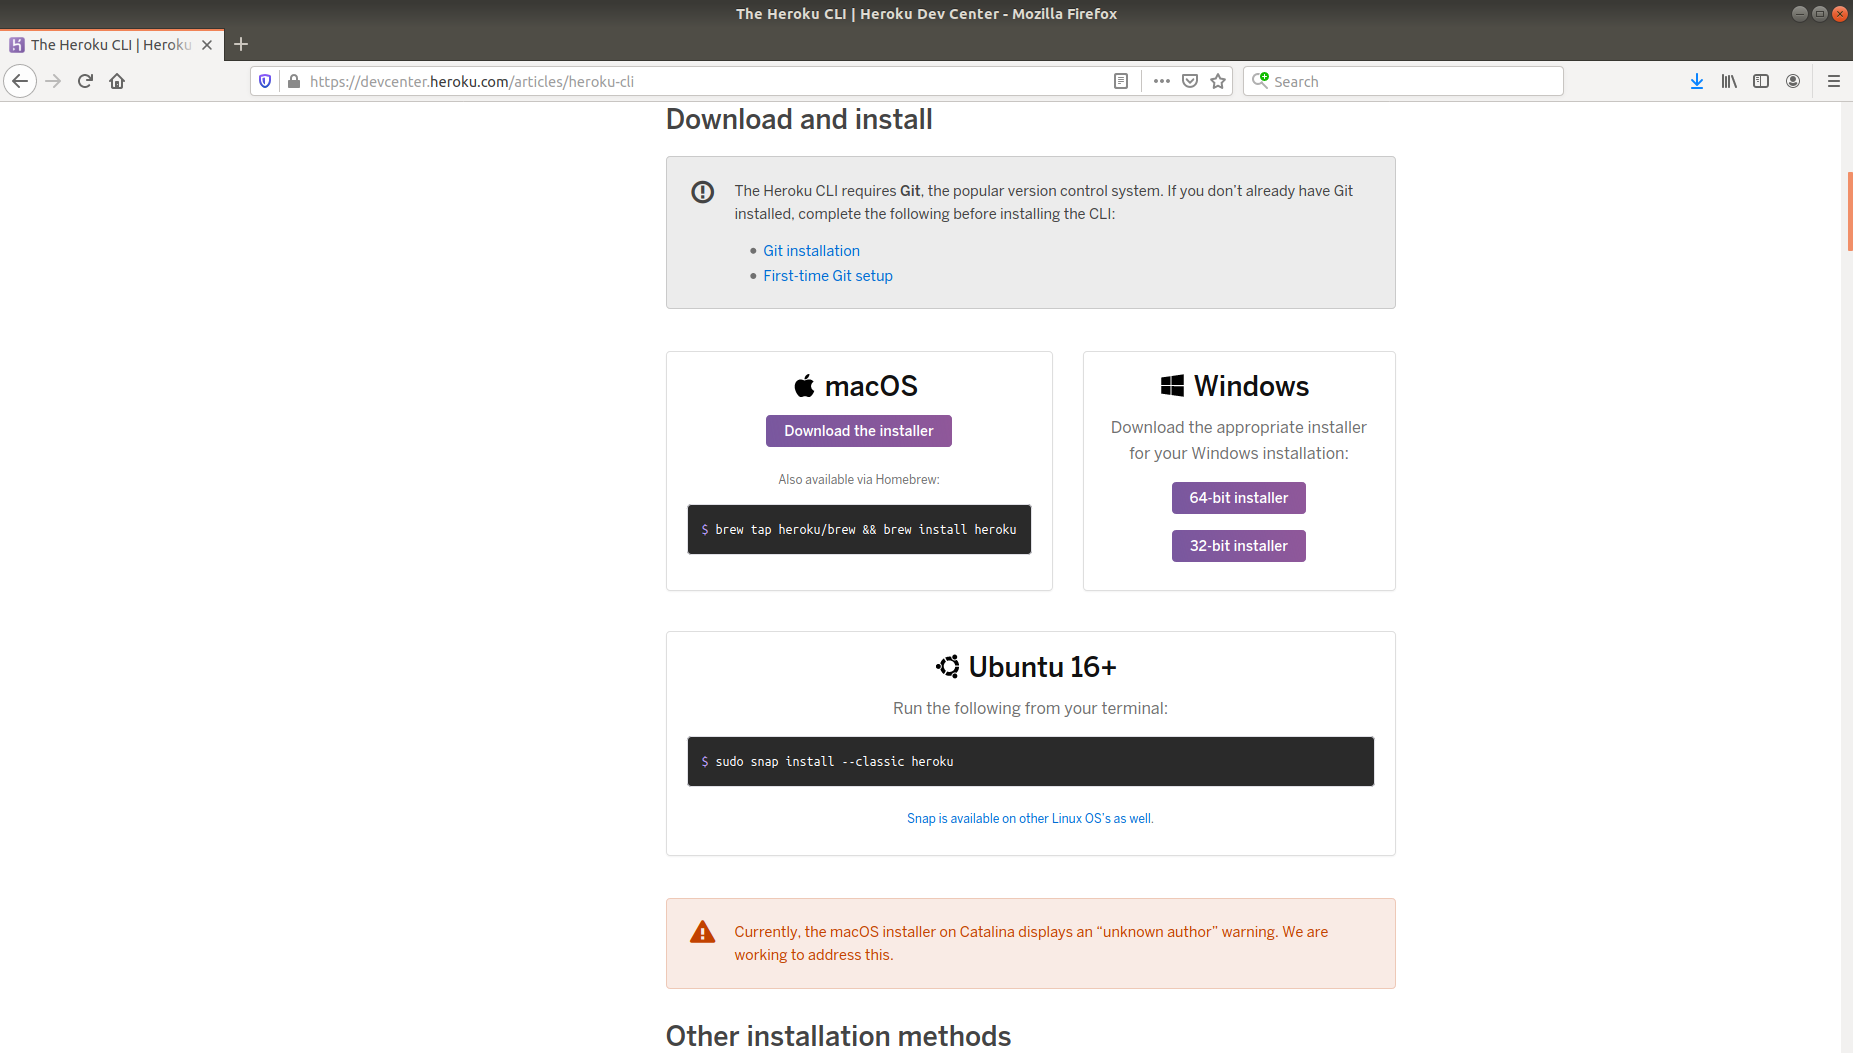
\includegraphics[scale=0.25]{slike/cliHeroku.png}
			 	\centering
			 	\caption{Instalacija Heroku CLI}
			 	\label{fig:promjene}
			 \end{figure}
			
			\newpage
			\textit{Nakon toga potrebno je napraviti novu aplikaciju klikom na gumb Create New App.}
			
			\begin{figure}[H]
				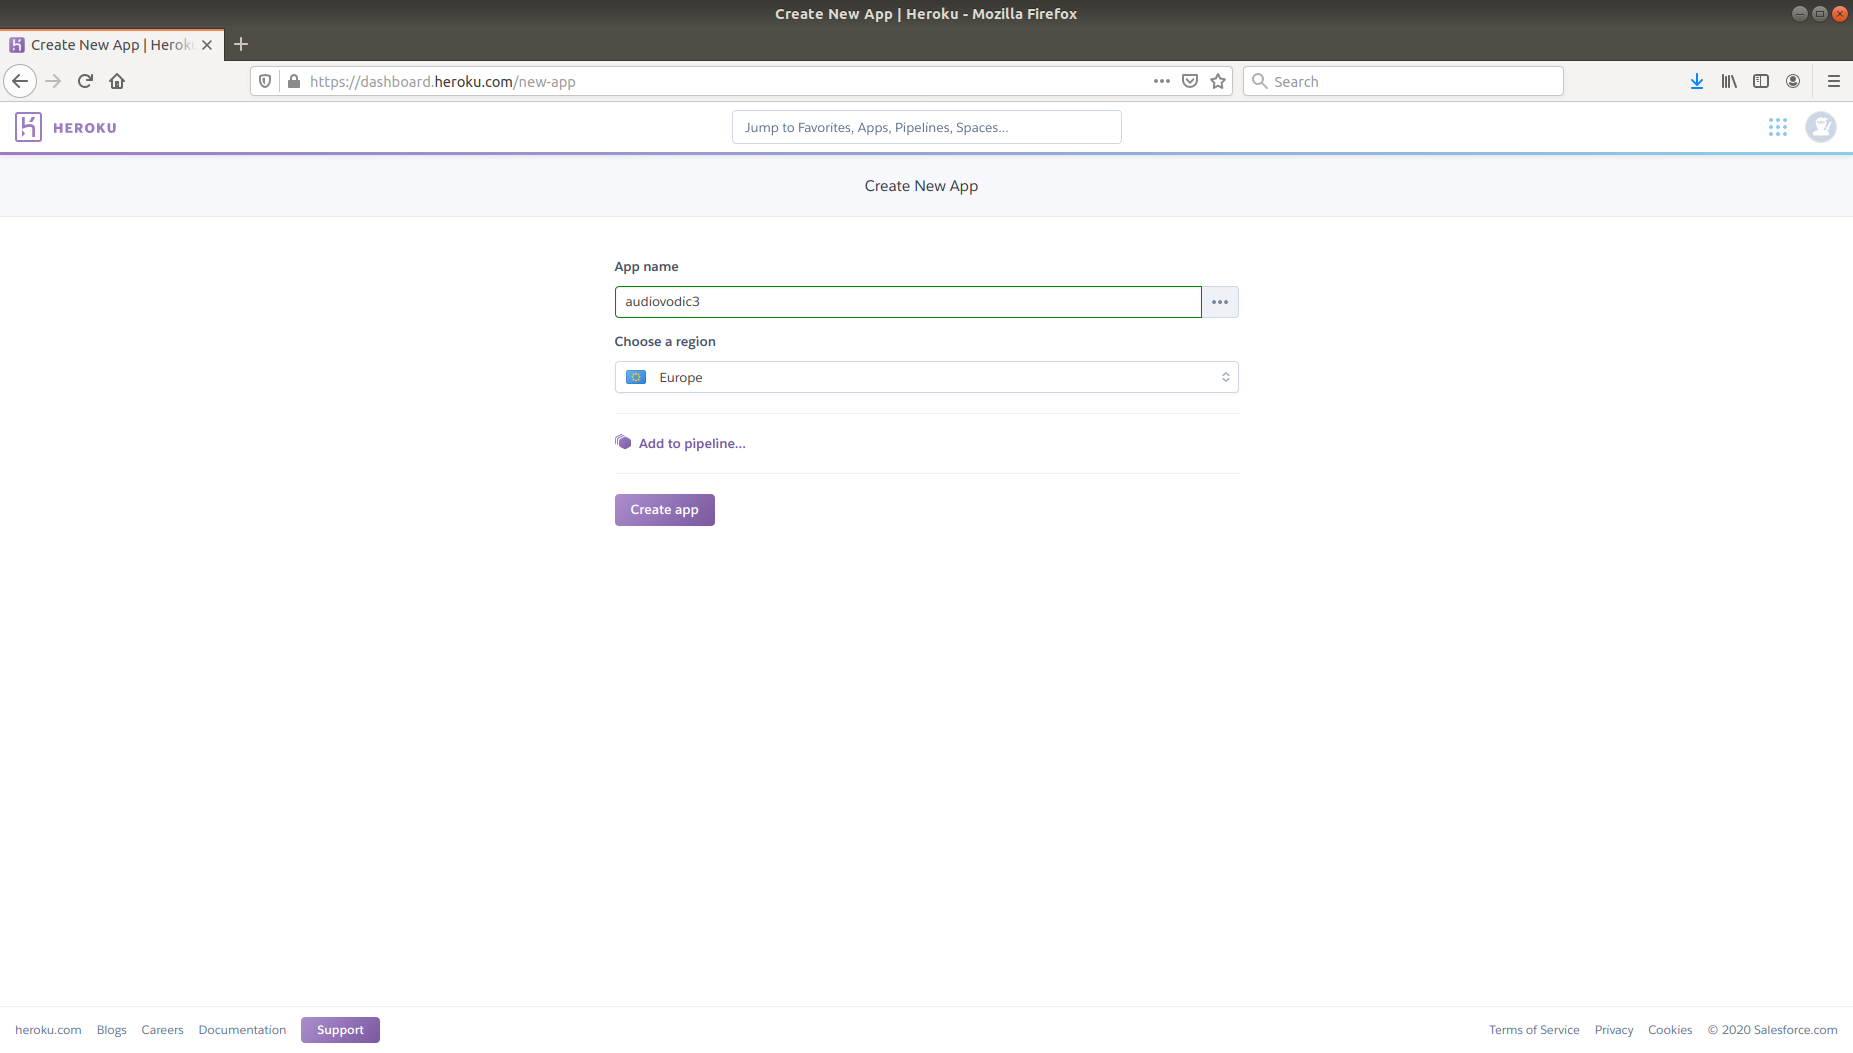
\includegraphics[scale=0.25]{slike/newHeroku.png}
				\centering
				\caption{Izrada nove aplikacije}
				\label{fig:promjene}
			\end{figure}
		
			\newpage
			\textit{Ako aplikacija sadrži bazu ili neki drugi resurs potrebno ih je sve dodati u izborniku Resources. U slučaju naše aplkacije potrebno je dodati Heroku Postgres u resources.}
			
			\begin{figure}[H]
				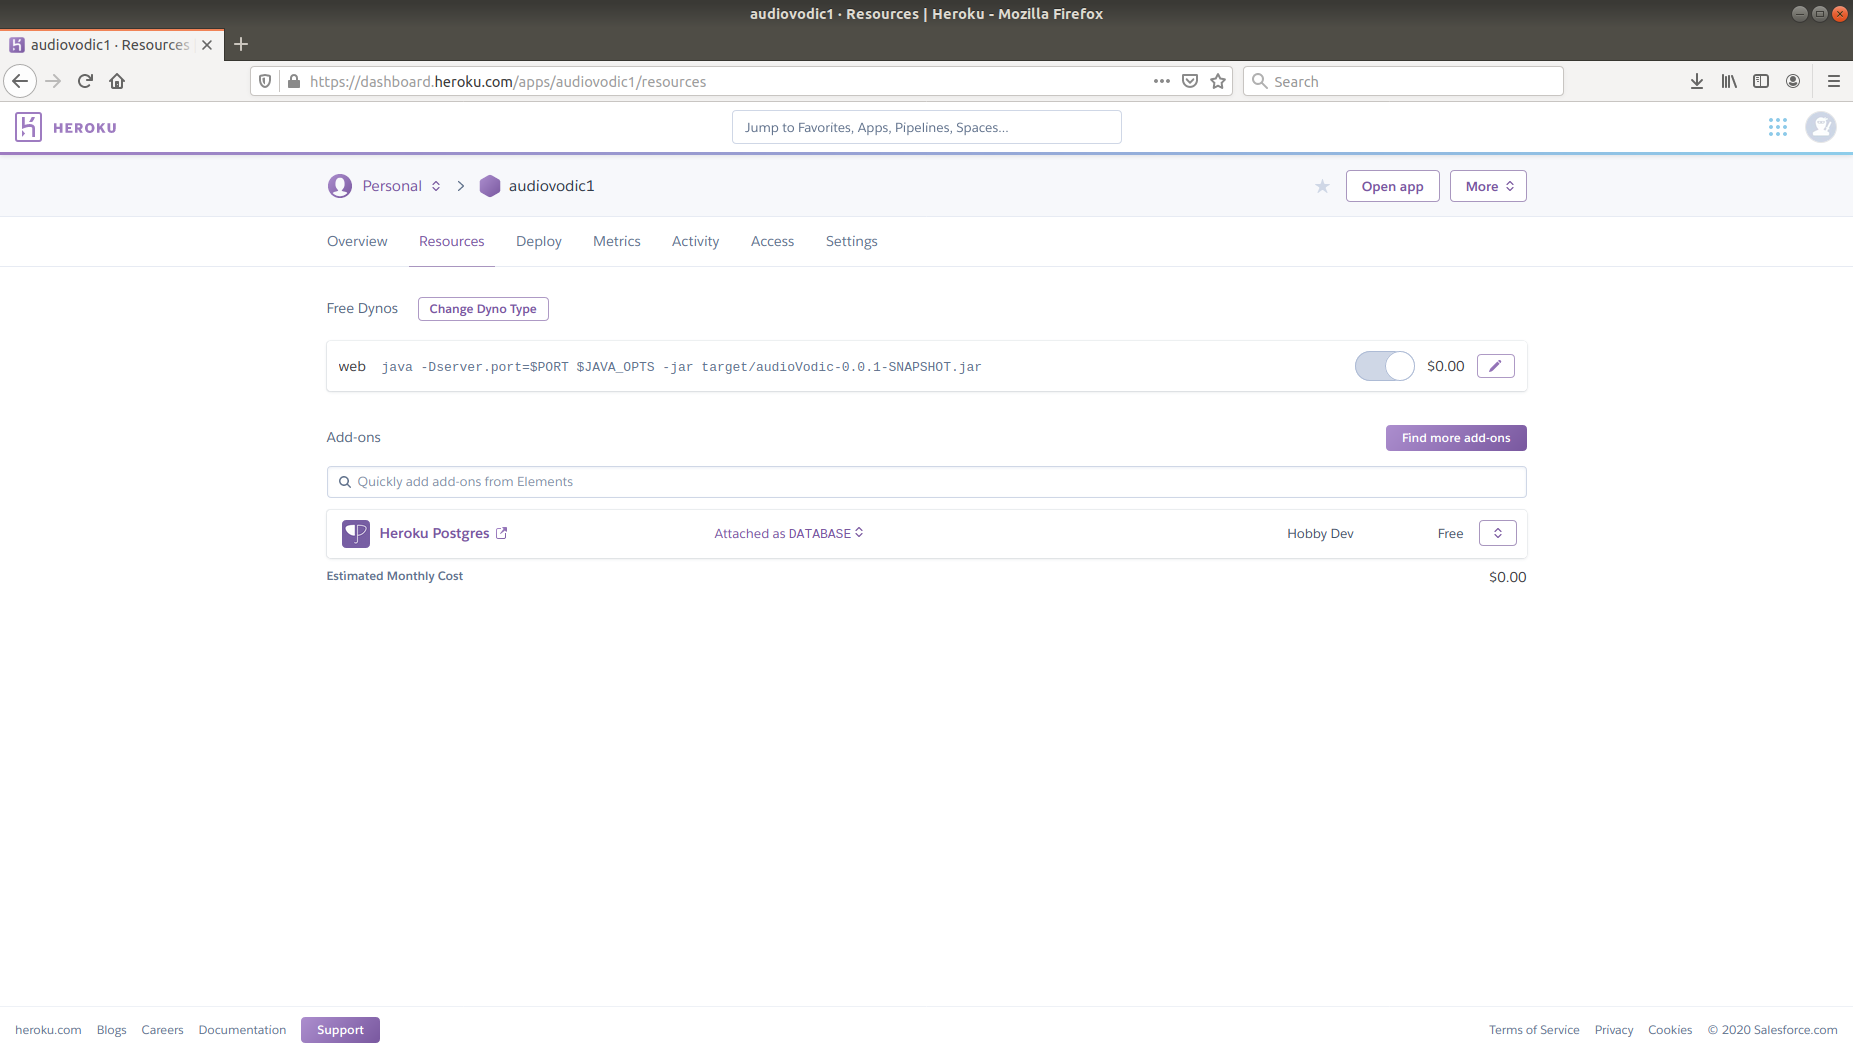
\includegraphics[scale=0.25]{slike/resHeroku.png}
				\centering
				\caption{Dodavanje resursa aplikacije}
				\label{fig:promjene}
			\end{figure}
		
			\newpage
			\textit{Zadnji korak je sam deploy aplikacije. Potrebno je otvoriti karticu deploy gdje se mogu naći naredbe potrebne za deployment aplikacije. Nakon što se izvrše naredbe korisniku se javlja je li aplikacije uspješno deployana. Ako je došlo do pogreške, korisniku se javlja koja se pogreška dogodila.}
			
			\begin{figure}[H]
				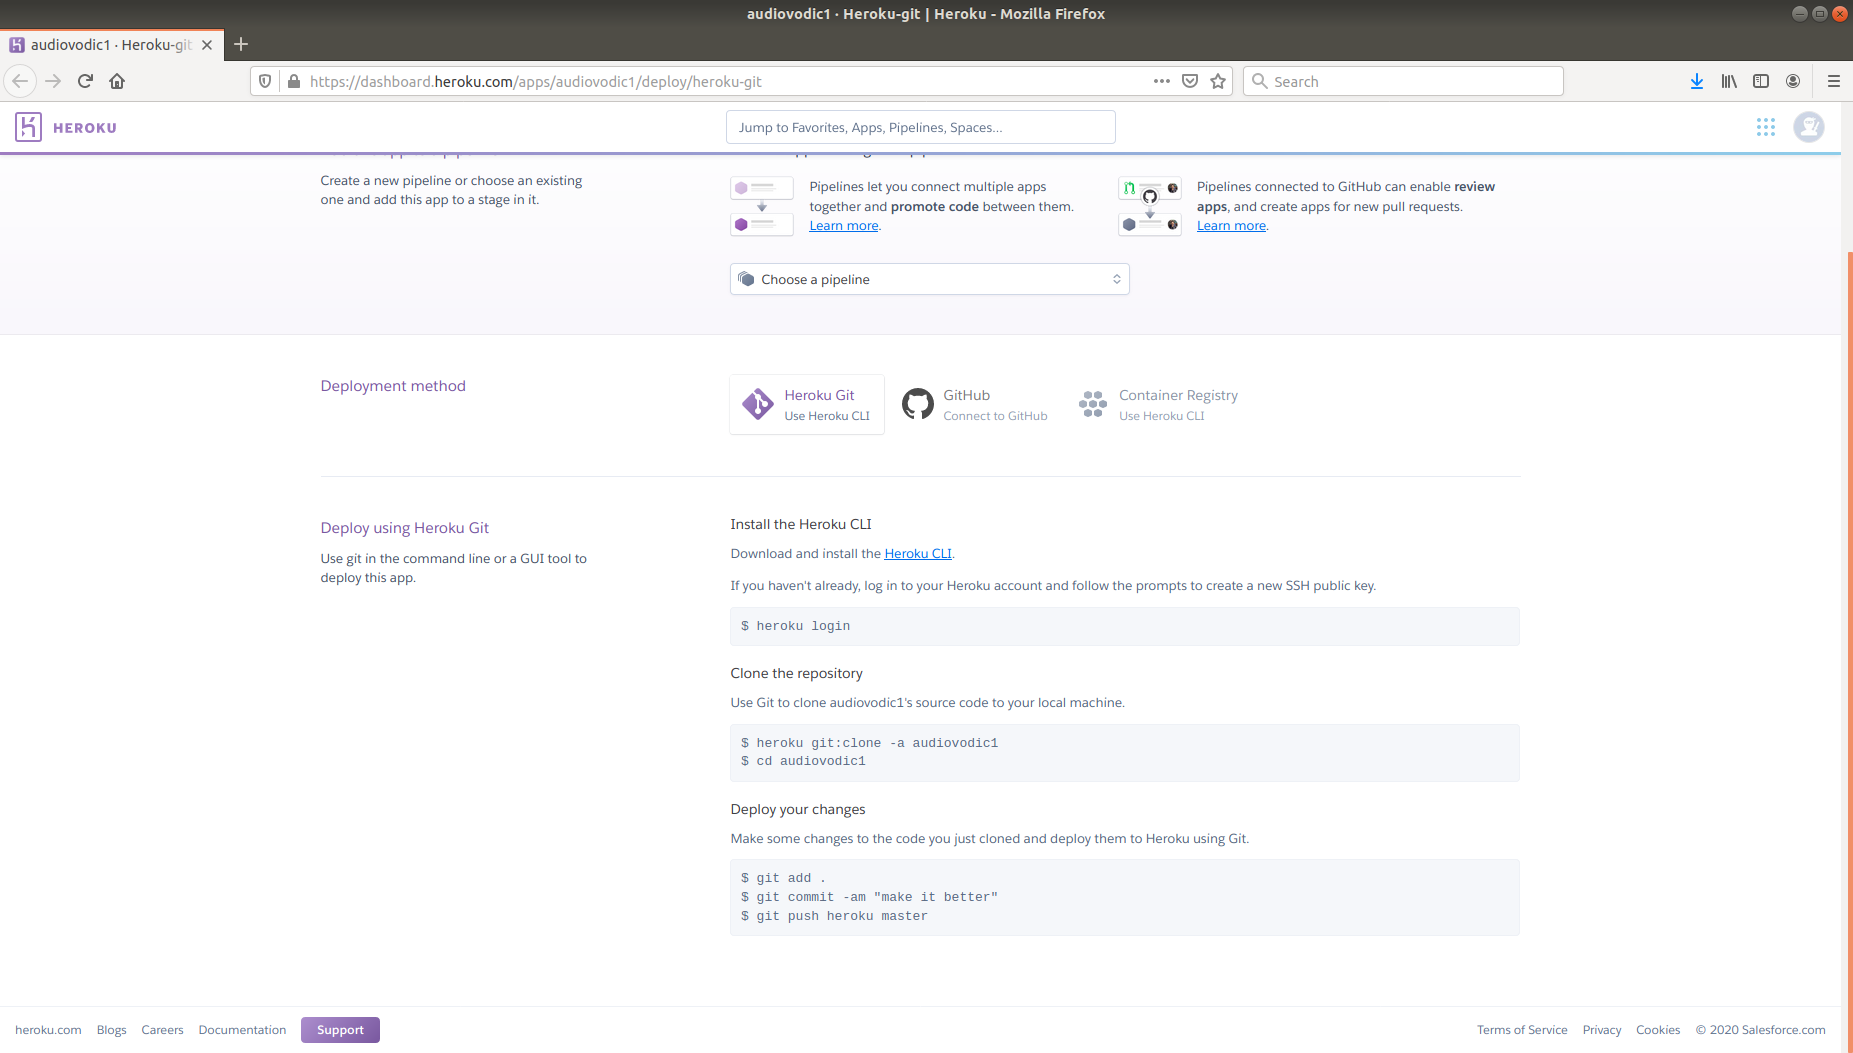
\includegraphics[scale=0.25]{slike/deployHeroku.png}
				\centering
				\caption{Deploy aplikacije}
				\label{fig:promjene}
			\end{figure}
			
			
			\eject 